% !TeX program = xelatex
\documentclass[UTF8,a4paper,11pt,fontset=fandol]{ctexart}
\usepackage[margin=2.25cm]{geometry}
\usepackage{amsmath,amssymb,bm,booktabs,longtable,array}
\usepackage{graphicx,subcaption,float,placeins}
\usepackage{xcolor,hyperref,fancyvrb,fvextra}
\hypersetup{colorlinks=true,linkcolor=blue!55!black,urlcolor=blue!55!black,
  pdftitle={科学机器学习作业一：总能量守恒与二维对流扩散降阶模型}}
\graphicspath{{figures/}}
\numberwithin{equation}{section}
\setlength{\parskip}{0.25em}
\setlength{\emergencystretch}{2em}
\captionsetup{font=small,labelfont=bf}
% Use TeX's expandable input inside alignments, avoiding LaTeX input lookahead.
\makeatletter
\let\TableInput\@@input
\makeatother
\newcommand{\vv}{\bm{v}}
\newcommand{\nn}{\bm{n}}
\newcommand{\qq}{\bm{q}}
\newcommand{\dd}{\mathrm{d}}
\newcommand{\cc}{\bm{c}}
\newcommand{\GridX}{200}
\newcommand{\GridY}{200}
\newcommand{\GridDx}{0.005}
\newcommand{\GridDy}{0.005}
\newcommand{\SnapshotCount}{151}
\newcommand{\StepCount}{4200}
\newcommand{\ActualDt}{0.00035714286}
\newcommand{\DtLimit}{0.00045454545}
\newcommand{\SnapshotInterval}{0.01}
\newcommand{\ResolutionNote}{当前数据已采用题目规定的空间网格；仍应独立核对实验与推导。}


\title{科学机器学习作业一\\[0.3em]
  \large 可压缩流体总能量守恒与二维对流扩散降阶模型}
\author{姓名：车保骏\qquad 学号：2501110040}
% \date{2026年10月18日}

\begin{document}
\maketitle

% \begin{abstract}
% 第一部分从固定控制体能量收支出发,推导无体力、无体热源的可压缩牛顿流体总能量方程,
% 区分能量输运、压力与黏性应力做功以及热传导.
% 第二部分采用单元中心有限体积法离散二维对流扩散方程,形成仿射系统
% $\dot{\cc}=A\cc+f$,并构建 POD--Galerkin 和保留常数坐标的投影增广 DMD.
% 基于现有 $\GridX\times\GridY$ 网格、$\SnapshotCount$ 个快照,比较
% $r=5,10,20$ 时四个指定时刻的浓度重构、相对误差、离散谱与空间模式.
% 默认实验使用整个计算时段训练,所得误差属于同轨迹重构误差.
% \textbf{\ResolutionNote}
% 本稿由 AI 辅助生成,提示词、现有实验材料及个人工作记录见附录.
% \end{abstract}

\section{问题一：可压缩 Navier--Stokes 总能量方程}

取任意固定区域 $V$,边界外单位法向为 $\nn$.记密度为 $\rho$、速度为 $\vv$、
单位质量内能为 $e$.单位体积的总能量为
\begin{equation}
  E=\rho e+\frac12\rho|\vv|^2.
\end{equation}
其中 $\rho e$ 是内能密度, $\rho|\vv|^2/2$ 是动能密度,两者相加得到总能量密度.
题目给出的应力矩阵和热通量分别为
\begin{equation}
 \bm{\sigma}=-pI+\bm{\tau},\qquad \qq=-\kappa\nabla T.
\end{equation}
这里 $p$ 是压力,$\bm{\tau}$ 表示黏性作用,$T$ 是温度,$\kappa$ 是导热系数.
矩阵 $\bm{\sigma}$ 作用在 $\nn$ 上,得到边界单位面积受到的力；
$\qq$ 表示热量流动的方向和大小,负号说明热量从高温处流向低温处.

区域内能量的变化来自三项：流体进出携带的能量、边界受力做功、热传导.
对应的量可写为
\begin{equation}
 \begin{aligned}
  \Phi_{\rm out}&=\int_{\partial V}E\vv\cdot\nn\,\dd S,
  &&\text{流体携带能量的净流出率},\\
  \dot W&=\int_{\partial V}\vv\cdot(\bm{\sigma}\nn)\,\dd S,
  &&\text{边界受力对区域内流体做功的功率},\\
  \dot Q&=-\int_{\partial V}\qq\cdot\nn\,\dd S,
  &&\text{热量的净输入率}.
 \end{aligned}
\end{equation}
第一项为正表示能量流出；第二项是通常的“力与速度内积”；
第三项中,$\qq\cdot\nn>0$ 表示向外传热,因此热输入率也要带负号.
没有体力和体热源时,能量守恒即“变化率等于净输入”,得到积分形式
\begin{equation}\label{eq:energy-balance}
 \frac{\dd}{\dd t}\int_V E\,\dd V
 =-\int_{\partial V}E\vv\cdot\nn\,\dd S
 +\int_{\partial V}\vv\cdot(\bm{\sigma}\nn)\,\dd S
 -\int_{\partial V}\qq\cdot\nn\,\dd S.
\end{equation}
由于本题应力矩阵对称,有 $\vv\cdot(\bm{\sigma}\nn)=(\bm{\sigma}\vv)\cdot\nn$.
代入应力和热通量,利用散度定理及区域 $V$ 的任意性,得到局部守恒形式
\begin{equation}\label{eq:energy-local}
 \frac{\partial E}{\partial t}
 +\nabla\cdot\big[(E+p)\vv-\bm{\tau}\vv-\kappa\nabla T\big]=0.
\end{equation}
括号内就是合并后的总能量通量,其中 $p\vv$ 来自压力做功.

\section{问题二：二维对流扩散与降阶模型}

\subsection{计算问题、数据来源与完成范围}
在 $\Omega=[0,1]^2$ 上求解
\begin{equation}
 \partial_t c+\partial_x c=D(\partial_{xx}c+\partial_{yy}c),
 \qquad D=0.01,\qquad c(0,x,y)=0.
\end{equation}
左边界为
\begin{equation}
 g(y)=c(t,0,y)=\begin{cases}1,&1/3<y<2/3,\\0,&\text{其他位置},\end{cases}
\end{equation}
上下使用周期边界条件,右侧 $\partial_x c(t,1,y)=0$.

\subsection{有限体积方法}
采用单元中心网格,$x_i=(i+1/2)\Delta x$、$y_j=(j+1/2)\Delta y$.
以 $c_{i,j}$ 表示单元平均浓度,物理数组按 $(j,i)$ 存储,向量编号为 $jN_x+i$.
正 $x$ 方向的内部总通量用迎风对流与中心扩散计算：
\begin{equation}
 F^x_{i+1/2,j}=c_{i,j}-D\frac{c_{i+1,j}-c_{i,j}}{\Delta x},
 \quad
 F^y_{i,j+1/2}=-D\frac{c_{i,j+1}-c_{i,j}}{\Delta y}.
\end{equation}
y 索引按周期循环.左侧边界面距离第一个单元中心仅为 $\Delta x/2$,因此
\begin{equation}
 F^x_{-1/2,j}=g_j-\frac{2D}{\Delta x}(c_{0,j}-g_j),
 \qquad F^x_{N_x-1/2,j}=c_{N_x-1,j},
\end{equation}
其中 $g_j=g(y_j)$.右侧通量只保留对流,外侧扩散通量为零.
半离散更新为
\begin{equation}\label{eq:fvm}
 \dot c_{i,j}=-\frac{F^x_{i+1/2,j}-F^x_{i-1/2,j}}{\Delta x}
 -\frac{F^y_{i,j+1/2}-F^y_{i,j-1/2}}{\Delta y}.
\end{equation}

令 $a=1/\Delta x$、$b=D/\Delta x^2$、$d=D/\Delta y^2$,
则式\eqref{eq:fvm}形成
\begin{equation}\label{eq:affine}
 \dot{\cc}=A\cc+f.
\end{equation}
内部单元的矩阵系数分别为
\begin{equation}
 A_{k,k}=-a-2b-2d,\quad A_{k,k-1}=a+b,\quad
 A_{k,k+1}=b,\quad A_{k,k\pm N_x}=d,
\end{equation}
跨越 y 边界的邻居按周期取值.左侧单元对角元为 $-a-3b-2d$,
右侧为 $-a-b-2d$,且
\begin{equation}
 f_{jN_x}=(a+2b)g_j,\qquad f_k=0\quad\text{对其他单元}.
\end{equation}
% 代码用 COO 汇总系数后转 CSR 存储 A,不构造全阶稠密矩阵.
% 内部面通量在相邻单元中符号相反,从而满足离散质量平衡；
% 本问题有入流和出流,区域内总质量本身不要求保持常数.

\subsection{时间步长与\texorpdfstring{$\delta t=0.01$}{dt=0.01}的分析}
显式 Euler 为
\begin{equation}
 \cc^{n+1}=\cc^n+\delta t(A\cc^n+f).
\end{equation}
为保持更新系数非负,采用包含边界单元在内的充分限制
\begin{equation}\label{eq:dt}
 \delta t\leq\frac{1}{\max_k(-A_{kk})}
 =\frac{1}{1/\Delta x+3D/\Delta x^2+2D/\Delta y^2}.
\end{equation}
这里不是仅分别考虑对流 CFL 或内部扩散条件,左侧半网格扩散还额外收紧了限制.
默认取上界的 $0.8$,再等分每个快照间隔,使保存时刻精确对齐.

由(\ref{eq:dt})计算出的网格上界为 $1/2200\approx4.5455\times10^{-4}$,实际采用步长为 $0.01/28\approx3.5714\times10^{-4}$,计算至 1.5 共执行 4200 次更新.
快照间隔 $\Delta t_s=\SnapshotInterval$,含初值共 $\SnapshotCount$ 列.

如果正式网格直接用 $\delta t=0.01$,它超过式\eqref{eq:dt}约 22 倍,
高频误差会剧烈放大.作为内区冻结系数的周期 Fourier 分析,取
$\theta_x=\theta_y=\pi$,放大因子为
\begin{equation}
 G=1-\delta t\left(\frac{2}{\Delta x}
 +\frac{4D}{\Delta x^2}+\frac{4D}{\Delta y^2}\right)=-35.
\end{equation}
这说明交替符号的短波误差具有很强的放大机制,可能出现振荡、负浓度并发散.

\subsection{全阶结果与四个时刻的空间分布}
表\ref{tab:fvm}给出面积加权总质量与浓度范围.
质量随入流增加,而出口逐渐建立流出；有限时间结果不能仅凭图像断言已经精确稳态.
\begin{table}[H]
 \centering
 \caption{现有 $\GridX\times\GridY$ 全阶结果.总质量为
 $\Delta x\Delta y\sum_{i,j}c_{i,j}$.}\label{tab:fvm}
 \begin{tabular}{cccc}\toprule
 $t$ & 总质量 & 最小浓度 & 最大浓度 \\\midrule
 \TableInput tables/fvm_statistics.tex
 \bottomrule\end{tabular}
\end{table}
图\ref{fig:c02}--\ref{fig:c15}同时给出 FVM、POD 和 DMD,以在同一色标下比较.
$t=0.2$ 时高浓度集中在左侧,$t=0.5$ 时输运至区域中部；
$t=1.0$ 时前沿接近出口,$t=1.5$ 时形成贯穿区域的带状分布.

\begin{figure}[p]\centering
 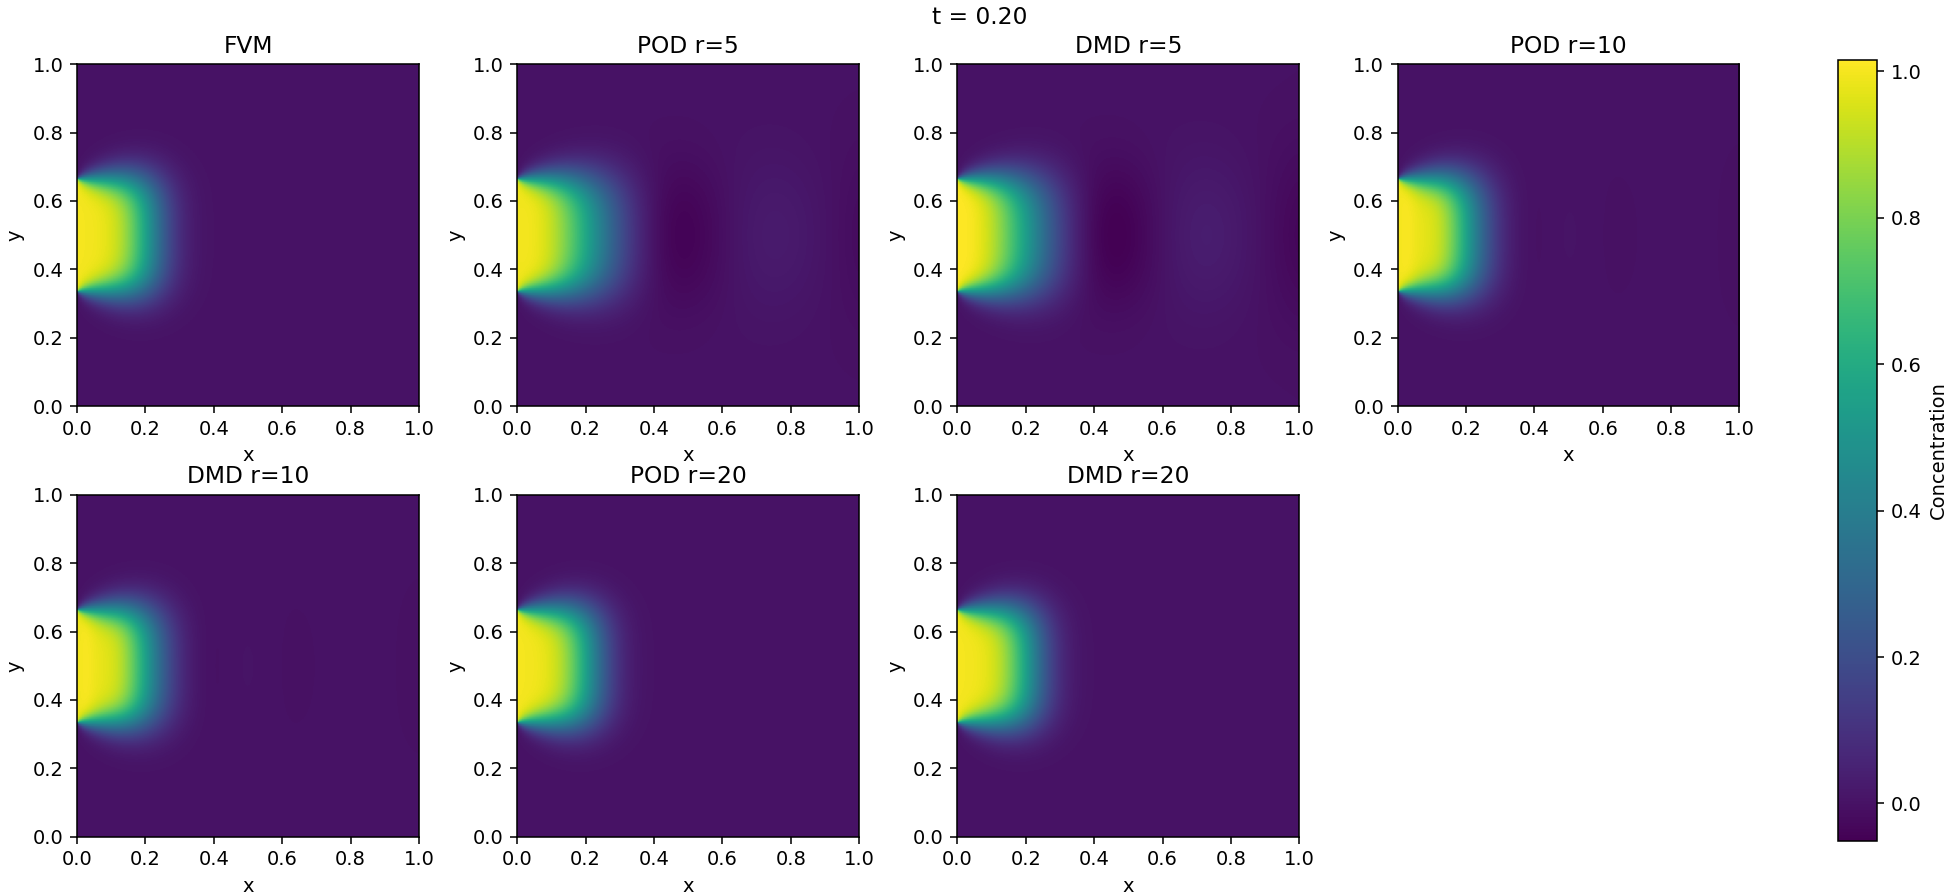
\includegraphics[width=0.97\textwidth]{concentration_t0.20.png}
 \caption{$t=0.2$ 的浓度比较}\label{fig:c02}
\end{figure}
\begin{figure}[p]\centering
 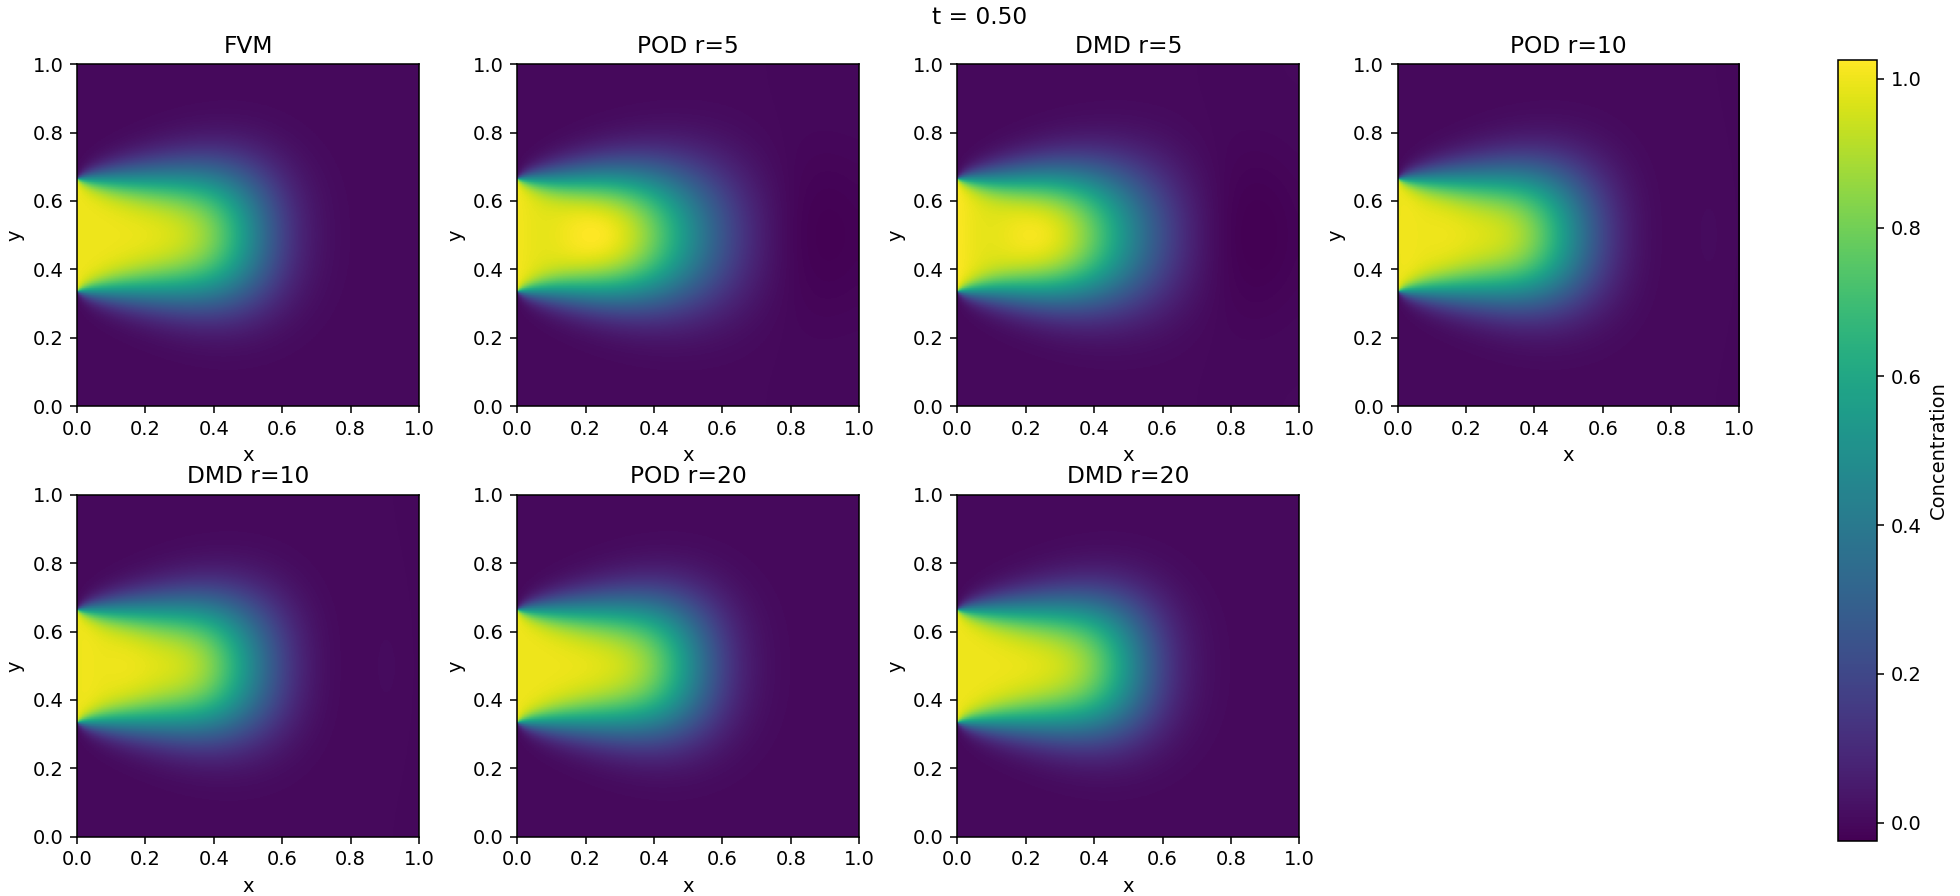
\includegraphics[width=0.97\textwidth]{concentration_t0.50.png}
 \caption{$t=0.5$ 的浓度比较}\label{fig:c05}
\end{figure}
\begin{figure}[p]\centering
 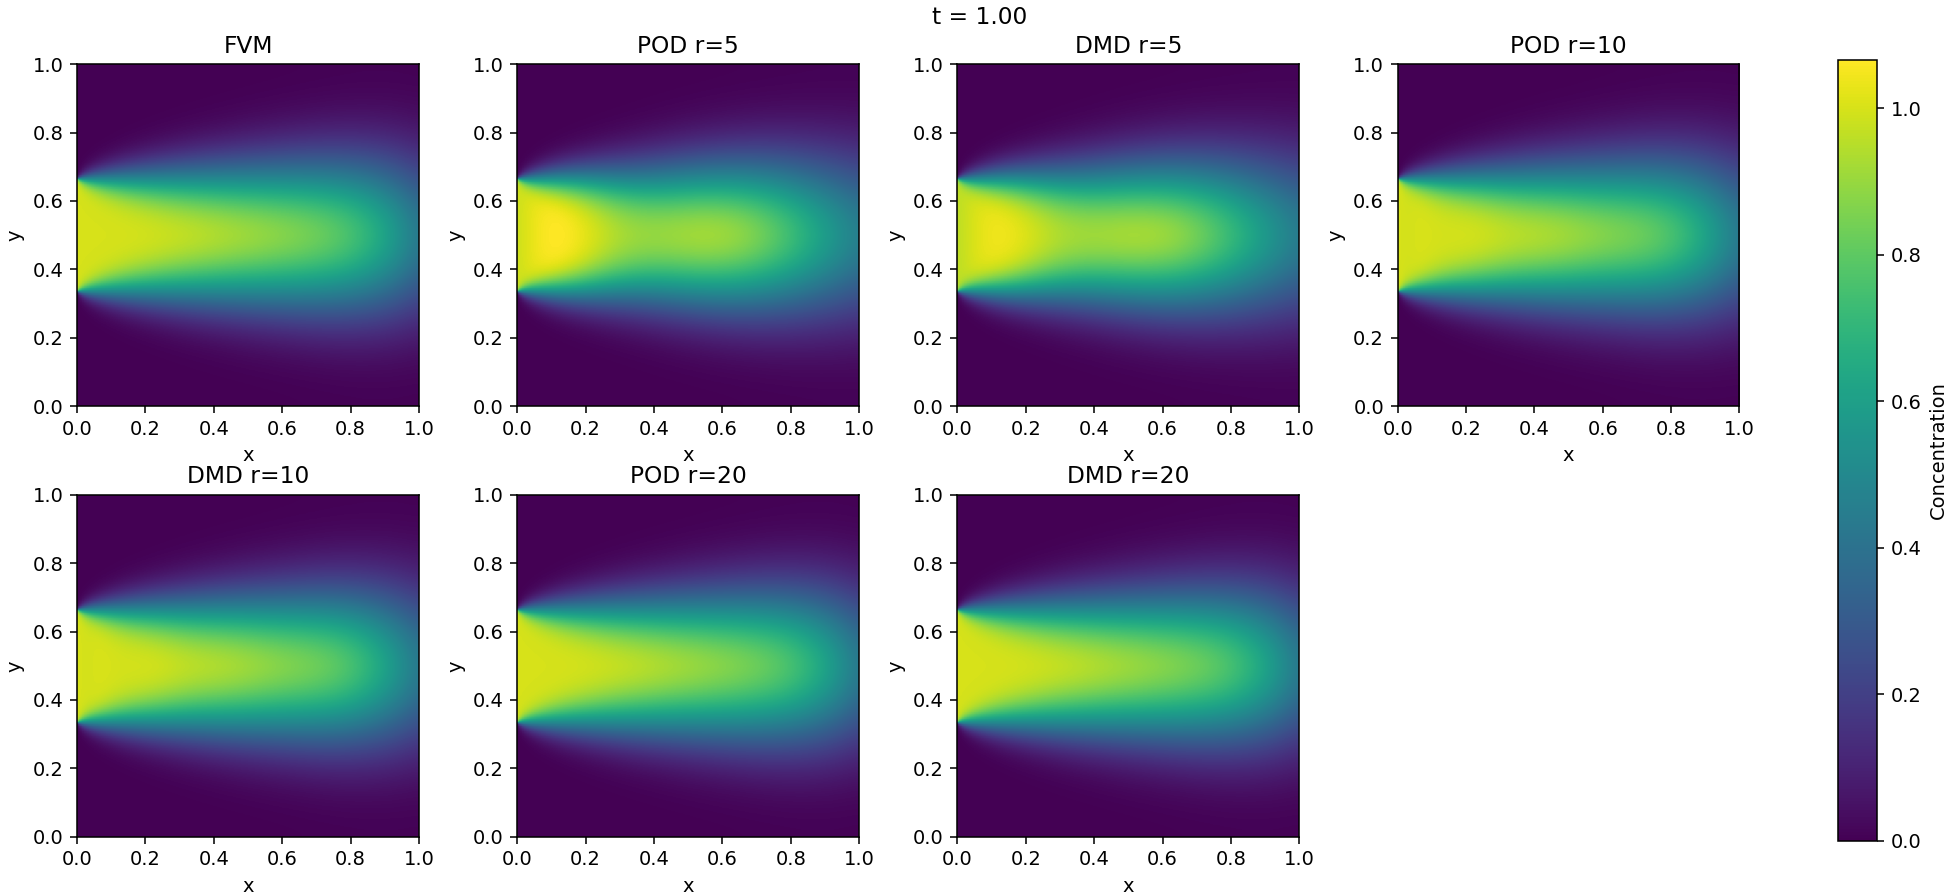
\includegraphics[width=0.97\textwidth]{concentration_t1.00.png}
 \caption{$t=1.0$ 的浓度比较}\label{fig:c10}
\end{figure}
\begin{figure}[p]\centering
 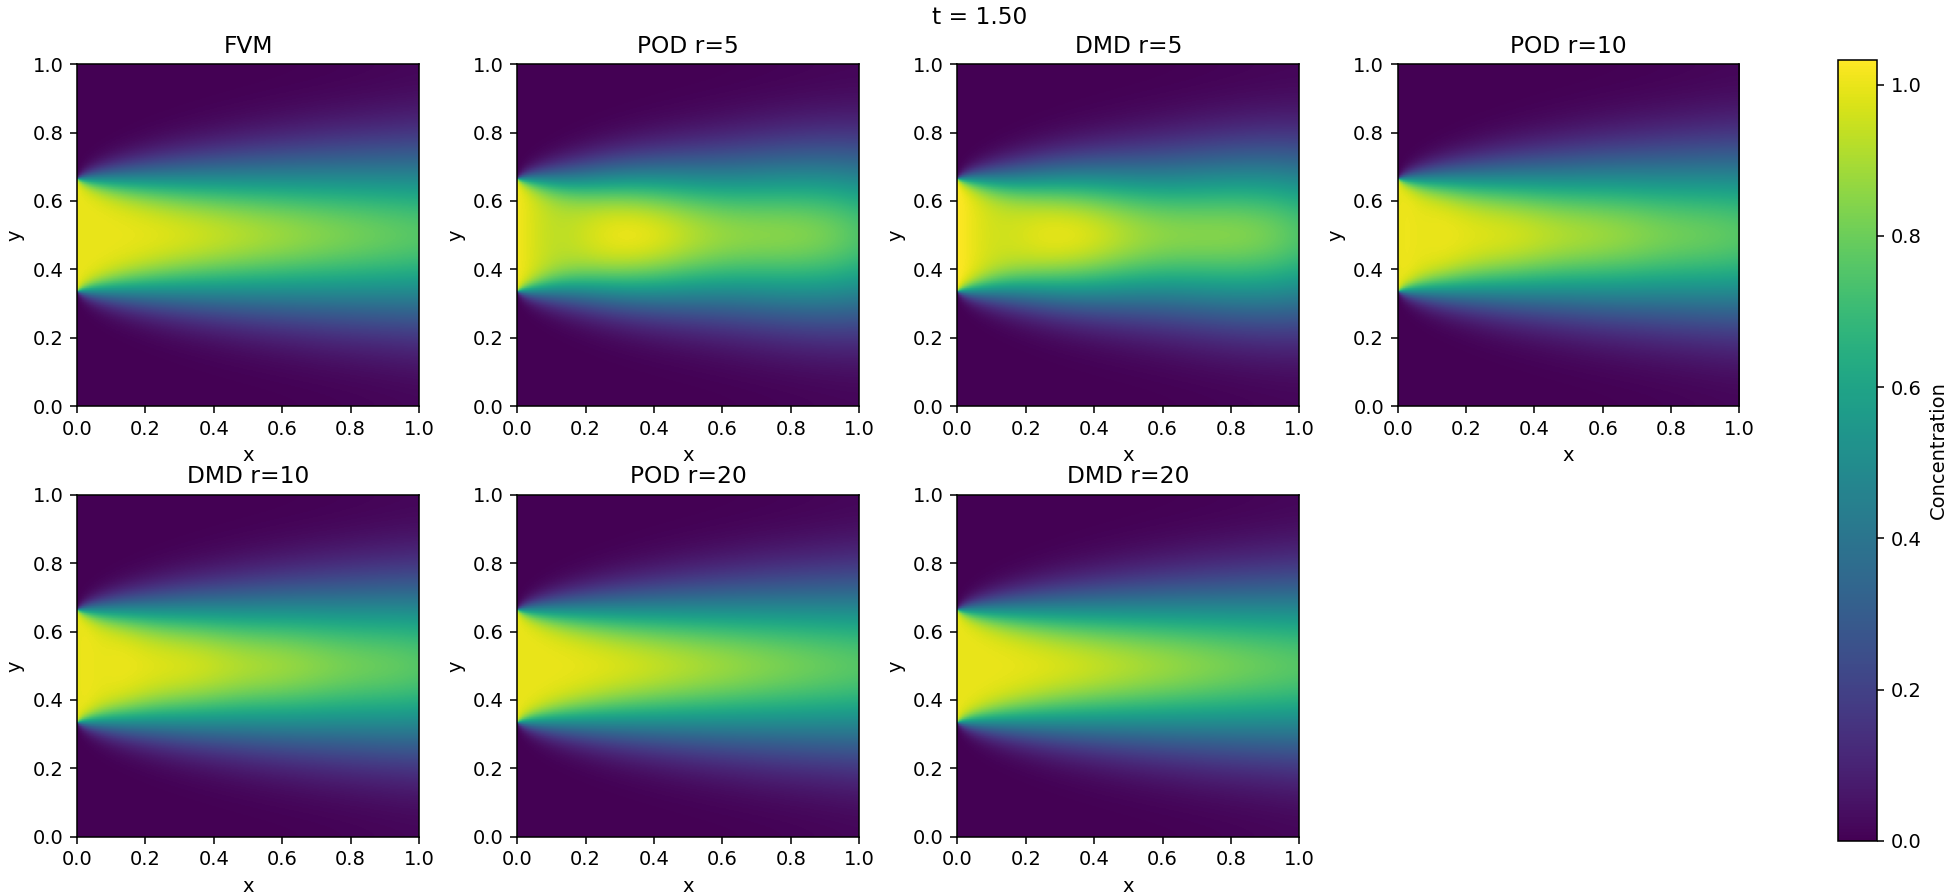
\includegraphics[width=0.97\textwidth]{concentration_t1.50.png}
 \caption{$t=1.5$ 的浓度比较}\label{fig:c15}
\end{figure}

\subsection{POD--Galerkin 降阶模型}
将全阶快照写为 $C=[\cc(t_0),\ldots,\cc(t_m)]$,作未中心化的薄 SVD：
\begin{equation}
 C=U\Sigma W^T,\qquad V_r=U(:,1:r),\qquad \cc\approx V_r a_r.
\end{equation}
$V_r^TV_r=I$.将式\eqref{eq:affine}投影到基底空间,得到
\begin{equation}\label{eq:pod}
 \dot a_r=A_r a_r+f_r,\quad A_r=V_r^TAV_r,\quad f_r=V_r^Tf,
 \qquad a_r(0)=V_r^T\cc(0)=0.
\end{equation}
POD(\ref{eq:pod})数值离散实现使用与全阶相同的实际 Euler 步长 $\ActualDt$.

% 默认 ,从零初值独立推进系数,
% 再以 $V_ra_r$ 重构全场.
% 对负实部特征值,显式 Euler 的特征值稳定条件为
% \begin{equation}
%  |1+\delta t\lambda|\leq1,\qquad
%  \delta t\leq\min_{\lambda\in\operatorname{spec}(A_r)}
%  \frac{-2\operatorname{Re}\lambda}{|\lambda|^2}.
% \end{equation}
% 表\ref{tab:pod}由现有降阶矩阵重新计算；它表明可研究较大 POD 步长,
% 但谱稳定不等于高精度,也不排除非正规算子的短时放大.
% \begin{table}[H]\centering
%  \caption{POD 快照累计能量与 Euler 特征值稳定上界.
%  能量指平方奇异值占比,不是总质量.}\label{tab:pod}
%  \begin{tabular}{ccc}\toprule
%  $r$ & $\sum_{i\leq r}s_i^2/\sum_i s_i^2$ & Euler 谱条件上界 \\\midrule
%  \TableInput tables/pod_diagnostics.tex
%  \bottomrule\end{tabular}
% \end{table}
% 累计能量很高仅说明整批数据容易被静态压缩,不保证所有时刻的动力学误差同样小.
% 未中心化的快照还包含平均分布的显著贡献.

\subsection{增广 DMD}
先用快照基底作 $z_k=V_r^T\cc_k$,再保留增广状态
$q_k=[z_k^T,1]^T$.
构造
\begin{equation}
 Z_-=[z_0,\ldots,z_{m-1}],\quad Z_+=[z_1,\ldots,z_m],\quad
 X_{\rm aug}=\begin{bmatrix}Z_-\\\bm{1}^T\end{bmatrix}.
\end{equation}
通过 SVD 最小二乘拟合
\begin{equation}
 [B\ b]=\arg\min_H\|Z_+-HX_{\rm aug}\|_F,
 \qquad K_{\rm aug}=\begin{bmatrix}B&b\\0&1\end{bmatrix}.
\end{equation}
最后一行固定,保证常数分量恒为 1.
预测采用
\begin{equation}
 q_k=K_{\rm aug}^{\,k}q_0,\qquad
 \cc_k^{\rm DMD}=V_r(q_k)_{1:r},\qquad
 k=(t-t_0)/\Delta t_s\in\mathbb{Z}_{\geq0}.
\end{equation}
DMD 每步跨越保存间隔 $\Delta t_s=\SnapshotInterval$,而不是 FVM 的内部积分步长.

对 $K_{\rm aug}w_\ell=\lambda_\ell w_\ell$ 求特征分解,
物理空间模式为 $\phi_\ell=V_r(w_\ell)_{1:r}$.
这些是所选观测空间中的离散 Koopman 谱与模式近似,
$|\lambda|<1$ 表示单个特征分量衰减,复相位对应振荡；
精确的 $\lambda=1$ 来自常数坐标,可携带稳态分布.

\begin{figure}[htbp]\centering
 \begin{subfigure}{0.32\textwidth}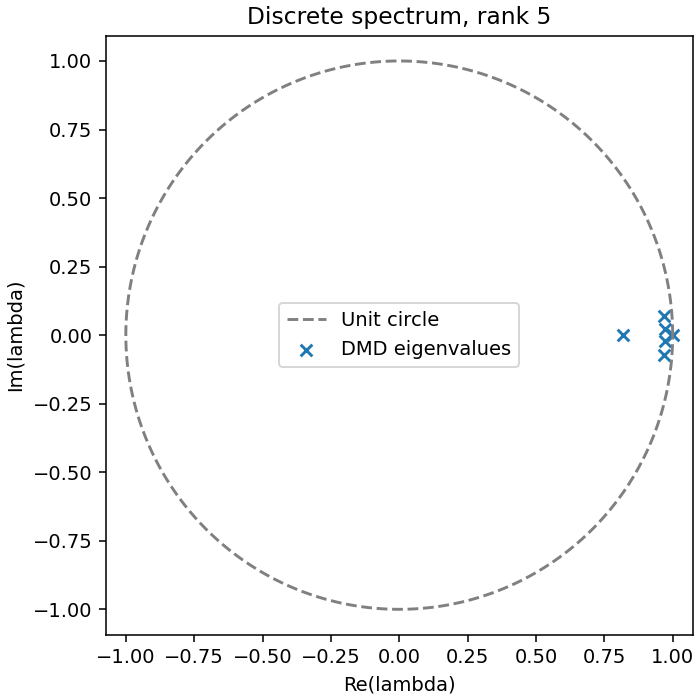
\includegraphics[width=\linewidth]{dmd_spectrum_r5.png}\caption{$r=5$,6 个特征值.}\end{subfigure}\hfill
 \begin{subfigure}{0.32\textwidth}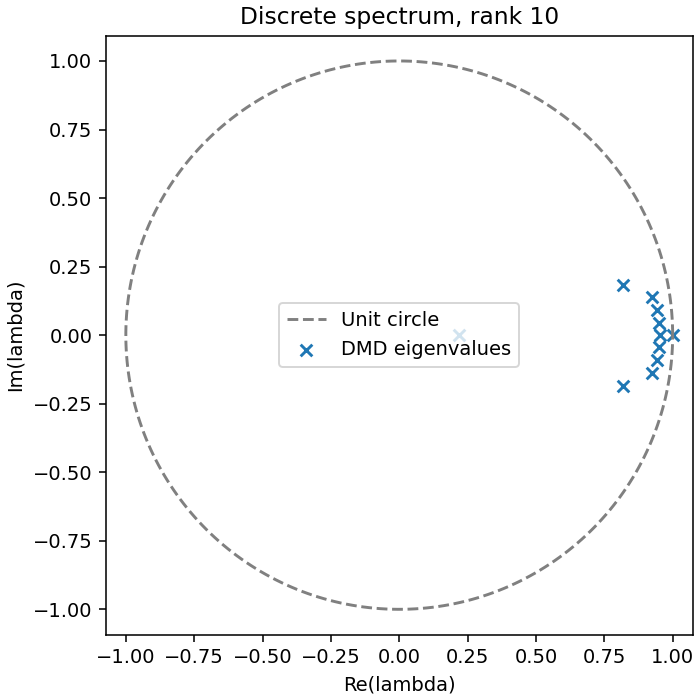
\includegraphics[width=\linewidth]{dmd_spectrum_r10.png}\caption{$r=10$,11 个特征值.}\end{subfigure}\hfill
 \begin{subfigure}{0.32\textwidth}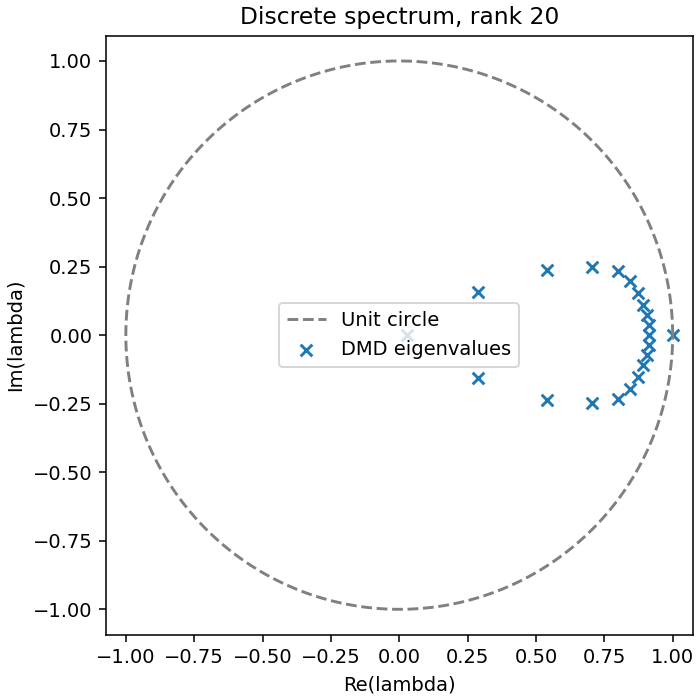
\includegraphics[width=\linewidth]{dmd_spectrum_r20.png}\caption{$r=20$,21 个特征值.}\end{subfigure}
 \caption{现有增广 DMD 的离散谱,灰虚线为单位圆.三组谱最大模均为 1,其余特征值在圆内.
 横纵轴为特征值实部与虚部,不是空间坐标；精确数值列于附录.}\label{fig:spectrum}
\end{figure}
主要空间模式见附录图\ref{fig:mode5}--\ref{fig:mode20}.

\subsection{四个时刻的误差与结果讨论}
以同网格 FVM 为参考,定义
\begin{equation}
 \|e(t)\|_{L^2_h}=\sqrt{\Delta x\Delta y\sum_k
  (c_k^{\rm ROM}(t)-c_k^{\rm FVM}(t))^2},\qquad
 \varepsilon_{\rm rel}(t)=\frac{\|e(t)\|_{L^2_h}}{\|\cc^{\rm FVM}(t)\|_{L^2_h}}.
\end{equation}
表\ref{tab:errors}覆盖两种模型、三种阶数和全部指定时刻.
\begin{table}[H]\centering\small
 \caption{正式 $\GridX\times\GridY$ 网格实验的相对误差$\varepsilon_{\rm rel}(t)$,参考为同网格全阶解.}\label{tab:errors}
 \begin{tabular}{cccccc}\toprule
 方法 & $r$ & $t=0.2$ & $t=0.5$ & $t=1.0$ & $t=1.5$ \\\midrule
 \TableInput tables/relative_errors.tex
 \bottomrule\end{tabular}
\end{table}
现有数据中,提高阶数显著减小误差：终止时刻 5 阶 POD 和 DMD 分别约为
$3.25\%$ 与 $2.24\%$,10 阶分别约为 $0.237\%$ 与 $0.209\%$,
20 阶则分别约为 $7.54\times10^{-6}$ 与 $7.39\times10^{-6}$ 的相对比例.
20 阶模型在终止时刻相近,但早期并不如此：$t=0.2$ 时,
POD 相对误差约为 $1.75\times10^{-3}$,DMD 约为 $1.25\times10^{-5}$；
$t=0.5$ 时分别约为 $8.18\times10^{-4}$ 和 $6.93\times10^{-6}$.
因此不能仅看最终时刻就判断两种方法在整个过程中等价,也不能据此推断 DMD 在其他问题上普遍更优.
两种方法都不强制浓度非负或不超过 1,例如 $t=0.5$ 的 POD 5 阶最小值约为
$-0.02267$、最大值约为 $1.02529$；$t=1.0$ 的最大值约为 $1.06558$,
说明较小全局误差也可能伴随局部过冲.

% 累计能量反映的是静态投影能力, POD--Galerkin 的误差还包括动力学闭合误差.
% 令 $P_r=V_rV_r^T$,真实轨迹的投影系数 $a_{\rm proj}=V_r^T\cc$ 满足
% \begin{equation}
%  \dot a_{\rm proj}=A_r a_{\rm proj}+f_r+V_r^TA(I-P_r)\cc.
% \end{equation}
% 降阶方程没有最后一项,即使 $(I-P_r)\cc$ 较小,经含空间导数的 A 作用后也未必可忽略.
% DMD 在当前完整训练轨迹上直接拟合保存时刻间的演化,可能取得不同的重构误差；
% 这不代表其在独立测试数据或改变边界条件后仍有同样优势.

% \begin{figure}[htbp]\centering
%  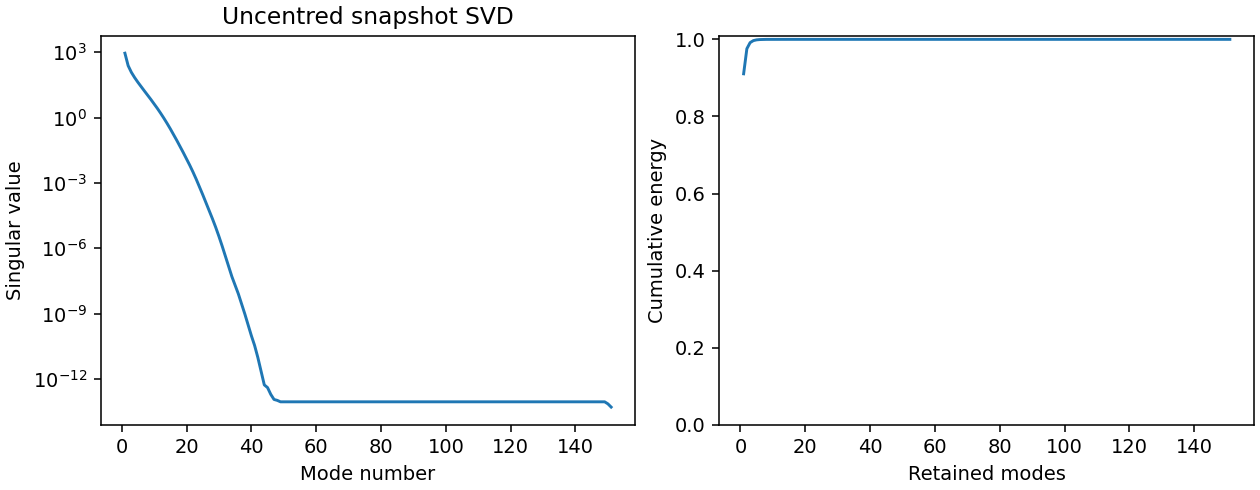
\includegraphics[width=0.92\textwidth]{pod_energy.png}
%  \caption{全部快照的奇异值衰减与累计能量.
%  奇异值尾部接近舍入误差水平,不宜解释为可靠的新物理结构.}\label{fig:energy}
% \end{figure}
% \begin{figure}[htbp]\centering
%  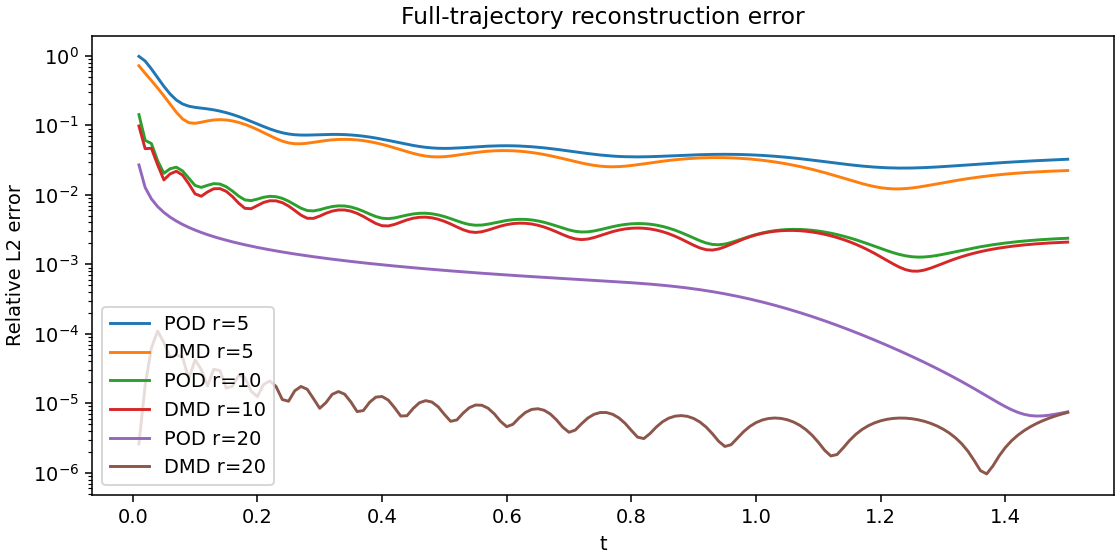
\includegraphics[width=0.92\textwidth]{errors.png}
%  \caption{全时段重构相对误差,纵轴为对数刻度.
%  初始时刻参考解为零,未绘入对数图；早期参考范数较小也会放大相对误差.}\label{fig:errors}
% \end{figure}
% \textbf{误差含义与限制：}所有快照都用于建基底或拟合,故这里没有独立测试时段.
% 小误差反映对当前 FVM 轨迹的重构能力,既不等于对连续方程精确解的误差,
% 也不证明换参数、换边界或长时间外推准确.
% 本次正式网格完整实验已完成；尚未进行网格/时间收敛研究、独立测试时段验证和可靠的运行时间加速比测试.

\subsection{怎样修改问题使固定低阶模型失效}
这里的失效指固定少量基底或固定训练映射的误差显著增大,
不是任意阶数的 POD/DMD 都必然无法表示修改后的问题.

一种修改是显著降低扩散,例如从 $0.01$ 降为 $10^{-4}$,
同时让窄入流条带的位置随时间移动,产生多个训练中未出现的尖锐平移前沿.
平移的局部尖峰往往不能被少量固定空间基底有效表示,快照奇异值可能衰减变慢；
旧 POD 基底会遗漏新结构,重新训练时也可能需要更多阶数.
这一修改还要求更细的全阶分辨率,避免把全阶数值扩散误认成 ROM 的性质.

另一种修改是将入流强度设为独立的时变输入 $u_b(t)$,并跨不同输入协议使用同一个模型.
离散方程变为 $\dot{\cc}=A\cc+f(t)$,不再具有固定 f.
对于相同当前浓度但不同后续输入,下一步状态不同；
单一、自治的 $[\cc;1]$ 映射无法同时表达这些演化,固定仿射 DMD 因而可能失效.
可考虑增加输入坐标、受控 DMD 或分时段模型；POD 也需要正确投影时变强迫并丰富训练集.

还可加入非线性反应,或改变速度方向.此时原先的固定线性闭合关系不再适用,
可能需要新的观测量、非线性降阶或重新训练.
若保留全部空间维数并正确投影修改后的完整方程,POD 只是坐标变换,
不应声称这种情况仍必然因降阶而失败.

\subsection{实现核验与复现入口}
% 实现用独立面通量检查稀疏矩阵、质量平衡、周期连接与左侧半网格边界,
% 并测试零状态、均匀稳态、稳定子步及准确保存时刻.
% POD 用完整基底核对与全阶积分等价；DMD 用已知仿射系统核对常数坐标、谱、模式与多步预测.
% 这些检查用于排除实现错误,不能替代正式分辨率和连续方程收敛验证.

在项目目录中运行以下命令可复现正式网格实验：
\begin{Verbatim}[fontsize=\small,breaklines=true]
python run_demo.py --formal --output outputs_formal
\end{Verbatim}
% 在 \texttt{report/} 目录运行以下命令,可从现有结果更新图表并编译报告：
% \begin{Verbatim}[fontsize=\small,breaklines=true]
% python prepare_report.py
% xelatex -interaction=nonstopmode -halt-on-error main.tex
% xelatex -interaction=nonstopmode -halt-on-error main.tex
% \end{Verbatim}
% 图表准备脚本默认读取上一级 \texttt{outputs\_formal/},不执行 PDE 求解.
% 图片、原始摘要/误差表副本和生成的表格分别保存在 \texttt{figures/}、\texttt{data/}、\texttt{tables/}.
% \FloatBarrier

\appendix
\section{增广 DMD 特征值明细}
下面列出原始模型全部特征值,按实部、虚部排序,保留 8 位小数.
复共轭对分别列出；每组多出的一个维数来自常数坐标.
\begin{longtable}{ccrrr}
 \caption{离散特征值,每步时间间隔为 $\SnapshotInterval$.}\label{tab:spectrum}\\
 \toprule $r$ & 序号 & $\operatorname{Re}\lambda$ & $\operatorname{Im}\lambda$ & $|\lambda|$ \\\midrule
 \endfirsthead
 \toprule $r$ & 序号 & $\operatorname{Re}\lambda$ & $\operatorname{Im}\lambda$ & $|\lambda|$ \\\midrule
 \endhead
 \bottomrule\endfoot
 \TableInput tables/dmd_spectrum.tex
\end{longtable}

\section{主要 DMD 空间模式}
每行是一个模式,左列实部、右列虚部,红/蓝表示模式正/负值.
实模式的虚部可能整片接近白色；这不是缺失计算.
同一行实部、虚部共享对称色标,不同行色标和复相位可能不同,不能仅凭颜色比较贡献.
\begin{figure}[!htbp]\centering
 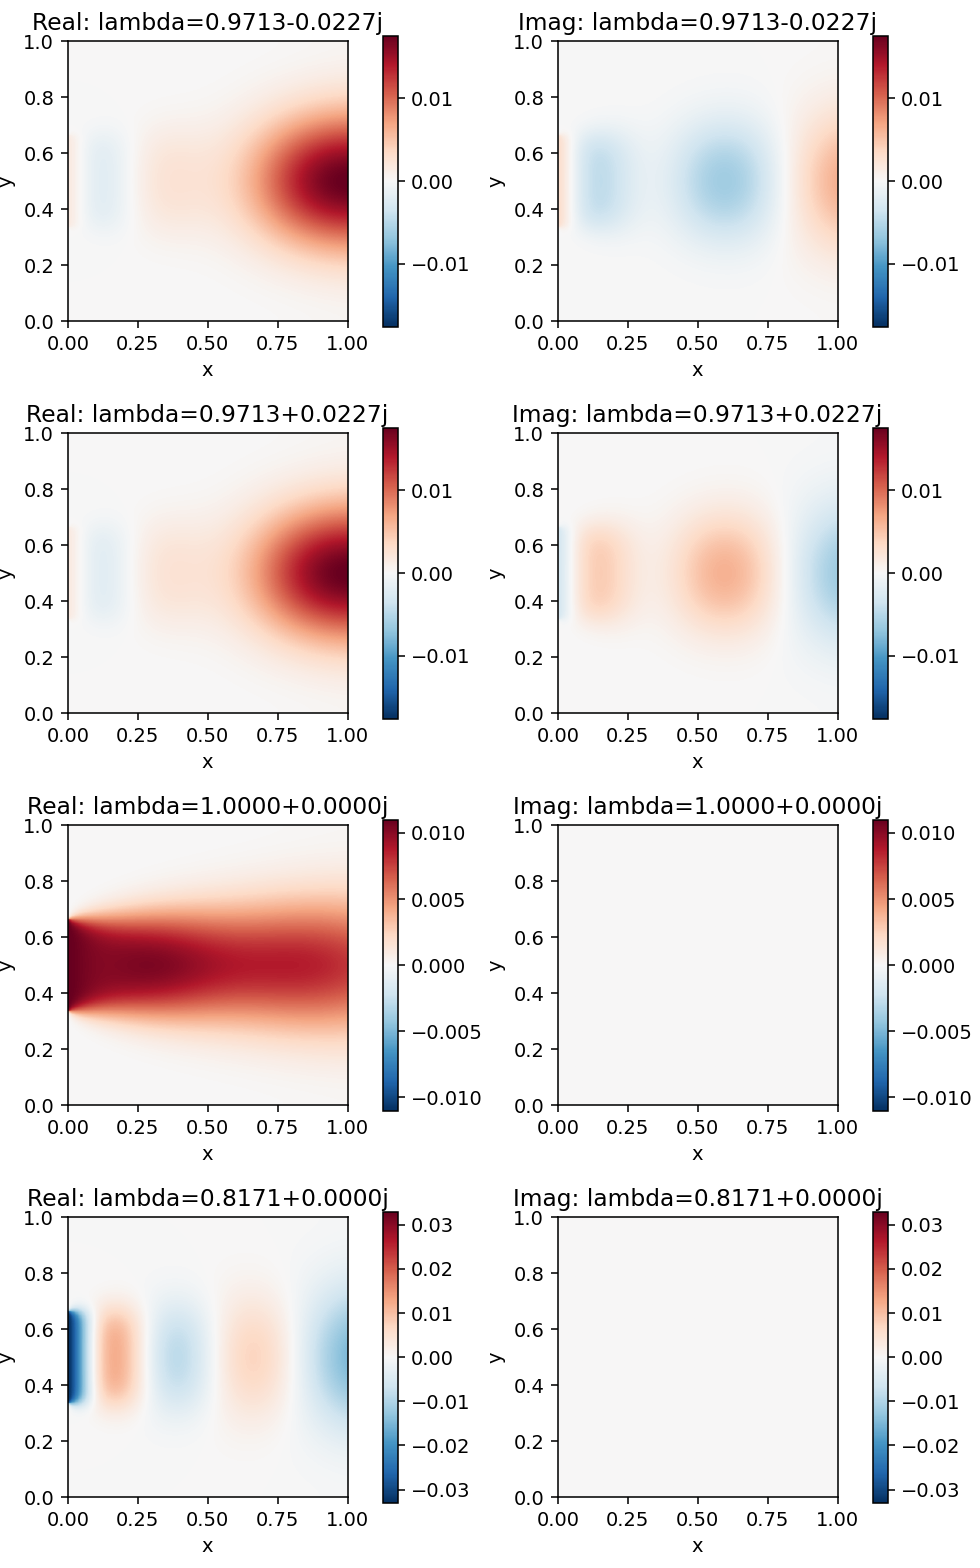
\includegraphics[height=0.70\textheight,keepaspectratio]{dmd_modes_r5.png}
 \caption{5 阶浓度空间对应的增广 DMD 主要模式.
 共轭模式的实部可相同、虚部符号相反；$\lambda=1$ 的模式可承载稳态结构.}\label{fig:mode5}
\end{figure}
\begin{figure}[p]\centering
 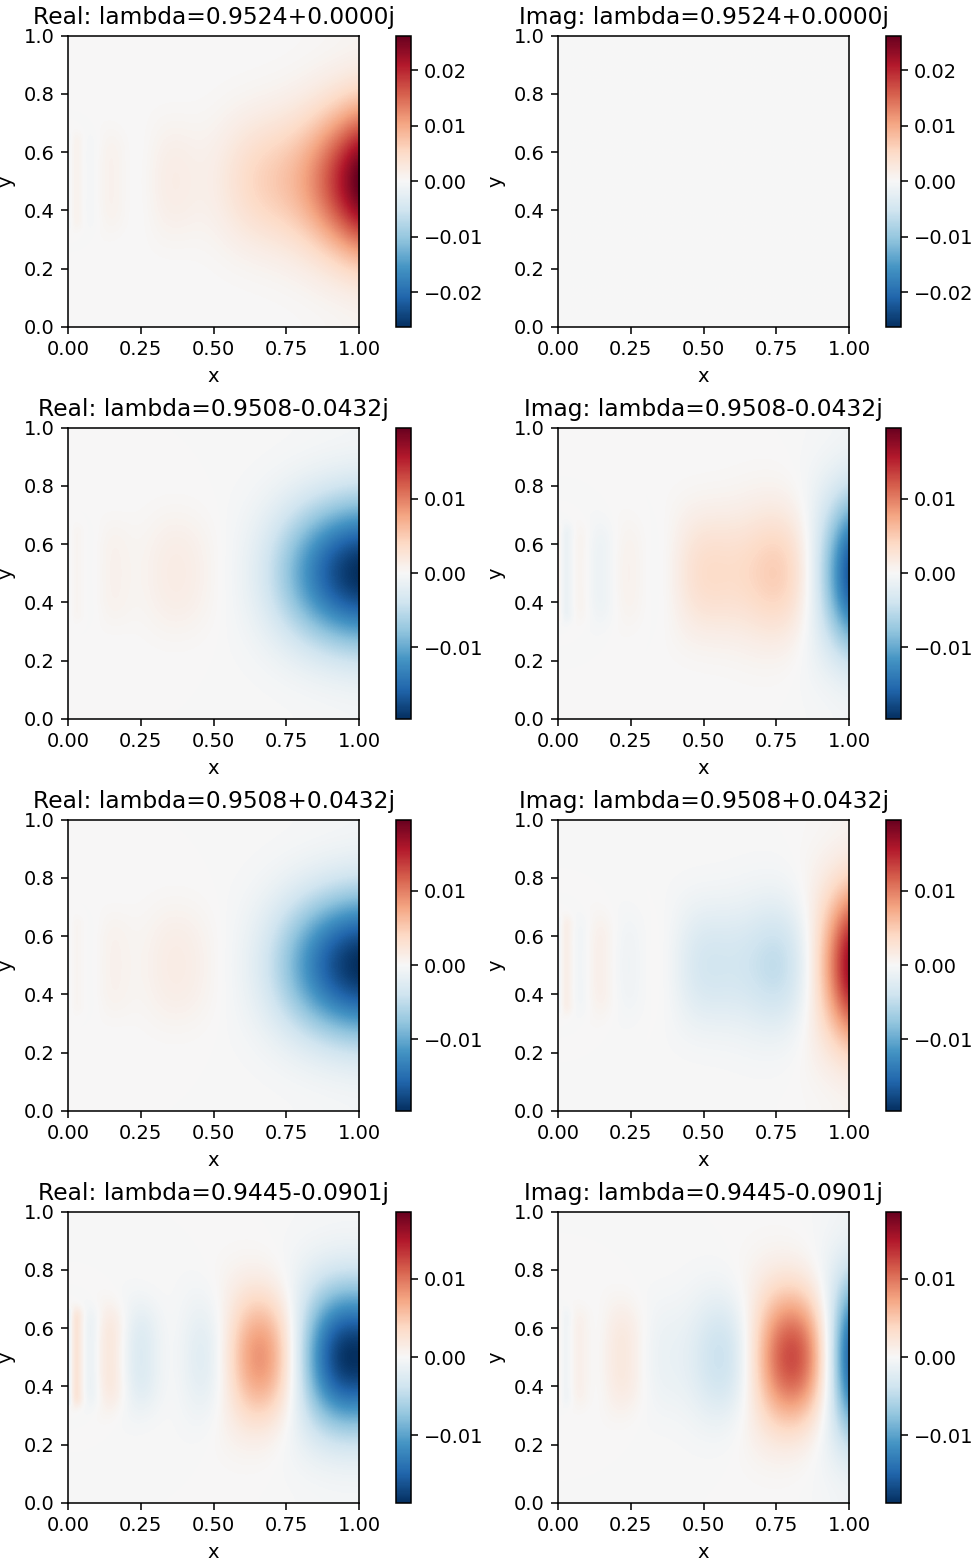
\includegraphics[height=0.76\textheight,keepaspectratio]{dmd_modes_r10.png}
 \caption{10 阶增广 DMD 的 4 个展示模式.模式不是某个时刻的浓度,负值允许存在.}\label{fig:mode10}
\end{figure}
\begin{figure}[p]\centering
 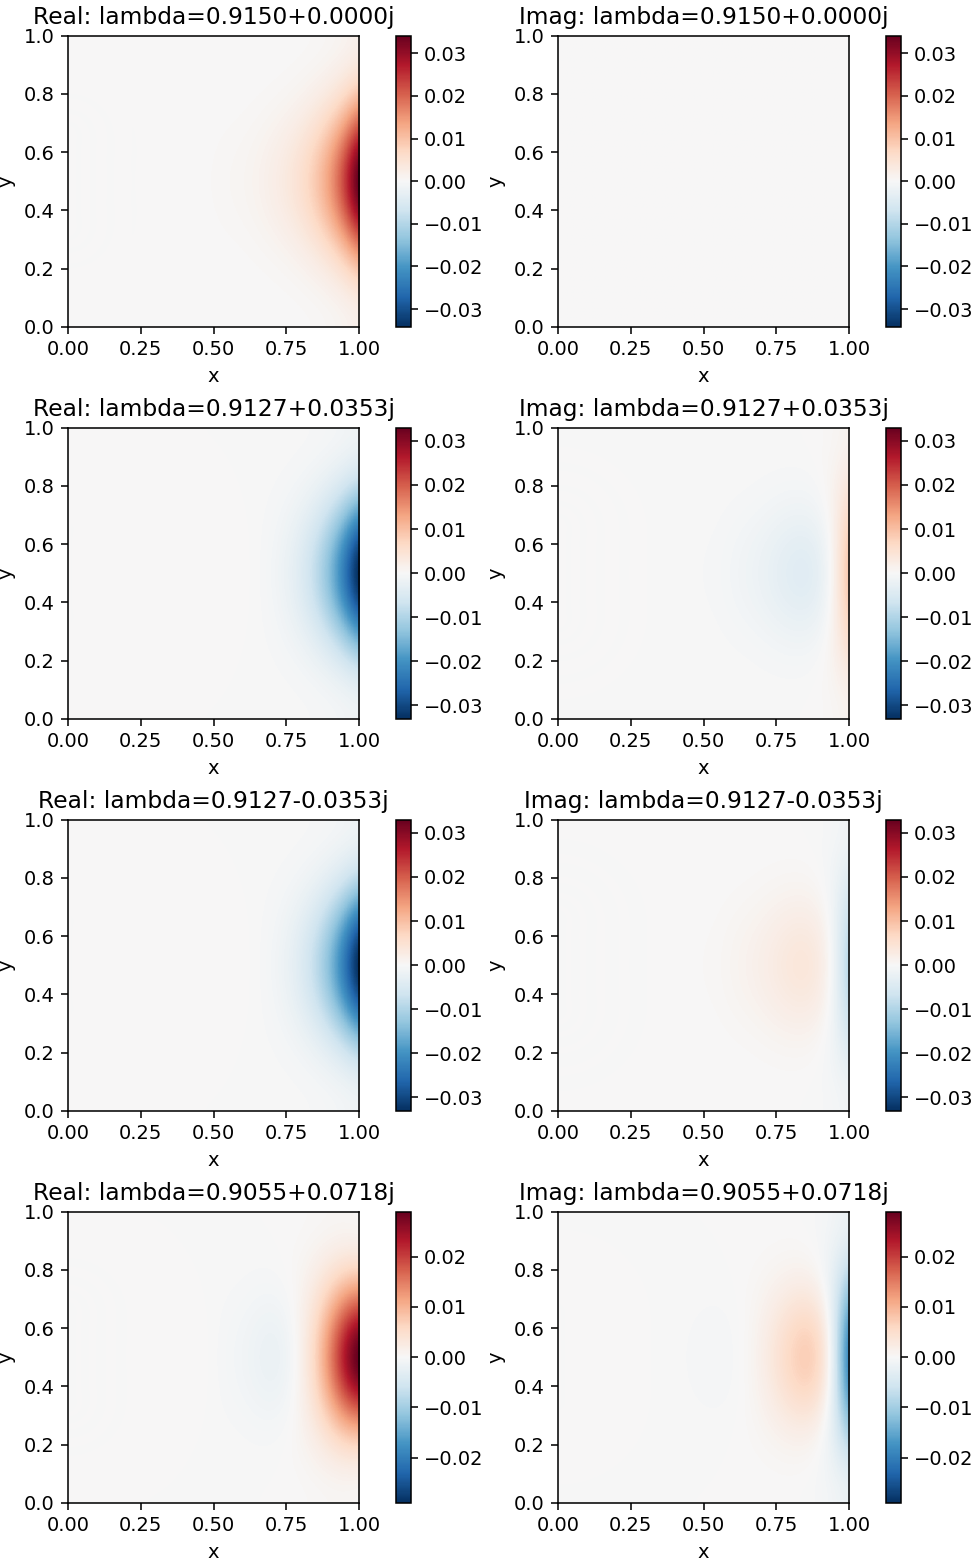
\includegraphics[height=0.76\textheight,keepaspectratio]{dmd_modes_r20.png}
 \caption{20 阶增广 DMD 的 4 个展示模式.完整模型有 21 个模式,
 根据初始幅度的展示排序可能没有选中 $\lambda=1$.}\label{fig:mode20}
\end{figure}
\clearpage

\section{AI 使用情况}
\textbf{本稿及部分基础程序由 OpenAI Codex 辅助生成.}
本稿第一题的推导检查和润色、第二题方法描述、文字分析、LaTeX 排版及数据表整理均由 AI 生成；
数值结果来自采用该 Python 基础代码生成的正式网格实验输出, 表格整理程序重新核对快照和 CSV.

主要用户提示词与决策包括：
\begin{enumerate}
 \item ``为我在Diffusion2D文件夹下,使用Python语言,初步完成 问题二:降阶模型上机练习 的基础代码,包括：实现问题的基本设置,几个算法的实现以及测试文件,以及一个md文件简要写做了什么,每个算法具体如何实现的.''
 \item 初版报告提示为：``基于现在这些结果,1. 为我写一下这个课程作业的latex报告的初稿.放在
 \texttt{Diffusion2D\textbackslash report} 文件夹下；2. 另外你觉得我还有什么可以自己调节和改进的地方？这些答案输出在这个聊天框.帮我批准所有增加文件的修改即可,不用问我太多.''
 \item 要求为基于新结果更新 LaTeX 报告,并删除两个辅助文本文件.
\end{enumerate}

% \begin{thebibliography}{9}
% \bibitem{assignment} 课程作业材料：\emph{科学机器学习作业一},题目一与题目二.
% \bibitem{implementation} 本地实现与实验记录：\texttt{diffusion2d/}、
% \texttt{run\_demo.py} 及 \texttt{outputs\_formal/}；本报告保存原始摘要和误差表的副本于 \texttt{data/}.
% \end{thebibliography}
\end{document}
